\chapter{El código abierto y libre} \label{chp:FOSS}

Este capítulo trata sobre qué es el código abierto y libre, \textit{\gls{FOSS}} por sus siglas en inglés\footnote{De \textit{Free and Open Source Software}.}, y qué importancia tiene actualmente tanto en entre el campo de investigación como en la industria.

Para poder comprender este trabajo más adecuadamente, se introducen algunos conceptos como \textit{\gls{issue}} o \textit{\gls{pull request}}, que se utilizan más adelante en las aportaciones planteadas en el \gls{repositorio}. En una línea más general, se tratará sobre la importancia de la \gls{documentación} y los procesos para poder aportar en un proyecto de este tipo.

\section{¿Qué es el código abierto y libre?} \label{sct:que_es_FOSS}

Los proyectos \textit{\gls{FOSS}} son aquellos donde una comunidad de desarrolladores publican el código en un \gls{repositorio} público y admiten que otras personas puedan proponer cambios y mejoras al mismo. Habitualmente se distribuyen bajo una \gls{licencia} que permite la modificación y redistribución del código y que hacen que su uso sea gratuito.

Esta clase de iniciativas suelen estar respaldadas por comunidades de desarrolladores que comparten un interés en común, o empresas que o bien se dedican a ello o facilitan que su personal aporte a estos proyectos.

El código abierto y libre tiene grandes éxitos y actualmente supone uno de los grandes pilares de la economía de \gls{software} \cite{dibona1999open, a556016d-4d87-3a33-80d5-87839d42cc50}. No es de extrañar la elevada calidad con la que cuentan \cite{Alenezi_Abunadi_2015} gracias a la colaboración e interés en el código que muestran las personas que lo respaldan.

Es más, en el ámbito de la investigación también se puede encontrar una gran cantidad de proyectos - hasta el punto de ser tema de publicaciones con recomendaciones sobre la gestión y el desarrollo \cite{10.1145/3472749.3474819}.

La elección de realizar este trabajo sobre código abierto y libre se debe especialmente a este compendio de razones, así como a que el resultado sea visible y accesible a cualquier interesado en el tema.

\section{Colaboración en proyectos \textit{FOSS}} \label{sct:colaboracion_FOSS}

Se ha mencionado anteriormente que dichas iniciativas se nutren de la colaboración entre múltiples personas -no solo desarrolladoras, sino también usuarias, entre otras- para identificar y producir mejoras, y mantener el proyecto. Es necesario por tanto establecer un marco de trabajo común sobre el que realizar estas aportaciones.

En general, cualquier proyecto de código con unos requisitos mínimos de calidad contará con un sistema de control de versiones (\gls{VCS}). Esta herramienta facilitará ver un historial de cambios, hacerlos de forma independiente pero simultánea entre desarrolladores, revisarlos, trazar errores y arbitrar los cambios que conforman cada nueva versión que se va publicando. Existen varios sistemas de control de versiones, como \textit{Mercurial} o \textit{Subversion}, pero el más popular y extendido es \textit{Git}; este último es el que se emplea en \pvlibpy{}.

Tradicionalmente estas propuestas se realizaban a través de listas de correo electrónico, pero actualmente se emplean plataformas como \textit{GitHub}, \textit{GitLab} o \textit{Bitbucket} que facilitan ver el código fuente y las propuestas con una \gls{interfaz gráfica} intuitiva. En el caso de \pvlibpy{}, se emplea \textit{GitHub}, una plataforma muy conocida por las iniciativas de código abierto y libre que pertenece al grupo \textit{Microsoft}.

Además, estas plataformas brindan una serie de características indispensables para la administración actual de proyectos:

\begin{itemize}
    \item \textit{Issues}: son temas de discusión que puedan tener un impacto concreto en el \gls{repositorio}. Aquí se suelen informar sobre los errores, posibles mejoras o tareas relacionadas en el proyecto. Cualquier persona con una cuenta en \textit{GitHub} puede abrir una \textit{\gls{issue}} y comentar en ella. Habitualmente se etiquetan para clasificarlos, priorizarlos y distinguir la fuente del error.
    \item \textit{Pull Requests}: son las propuestas con cambios que plantean desarrolladores del proyecto. Se pueden revisar, comentar y aprobar o rechazar. En la administración de un proyecto serio y riguroso como \pvlibpy{}, es un paso imprescindible para aportar cualquier cambio al código. Las propuestas pasan un proceso de revisión y triage para garantizar la calidad y asignarlas a una versión apropiada a la tipología del cambio.
    \item \textit{Discussions}: son foros para tratar cualquier tema, normalmente menos serios que una \textit{\gls{issue}}. Es uno de los lugares más apropiados para plantear dudas o sugerencias sin formalizar ni una aportación ni requerir la atención inmediata.
\end{itemize}

Todos los cambios que se proponen al código en este TFG se realizan a través de \textit{pull requests}, y en el caso de las propuestas más grandes se acompaña con frecuencia de una \textit{\gls{issue}} para discutir sobre la propuesta antes de realizarla.

Desde un punto de las interacciones sociales y las responsabilidades, es interesante definir las acciones que toma un desarrollador cuando va a realizar una propuesta:

\begin{figure}[H]
    \centering
    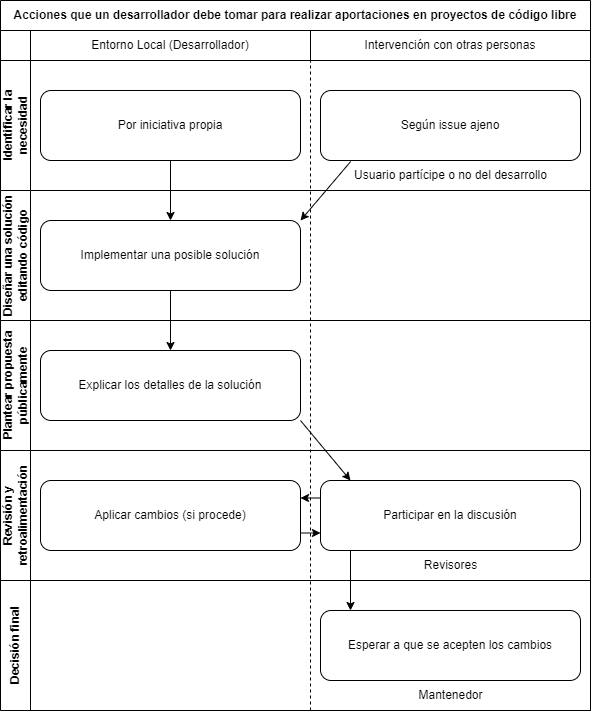
\includegraphics[width=0.8\textwidth]{images/SoA_foss/Contrib_dev.png}
    \caption{Diagrama de flujo de trabajo de un desarrollador en un proyecto \textit{FOSS}.}
    \label{fig:FOSS_workflow}
\end{figure}

De este flujo deben hacerse unas anotaciones importantes:

\begin{itemize}
    \item El rol de la persona que interviene en cada caso puede corresponder a una misma persona en varias ocasiones; este es el caso de los administradores del proyecto.
    \item A veces, en cada intervención hay más de una persona que toma el rol, en especial de quienes revisan.
    \item A partir de ``Plantear propuesta públicamente'' todos los cambios del historial que se hayan hecho son visibles para todo público. Por esta razón es importante cuidar que no se incluya información sensible en ningún momento.
\end{itemize}

\subsection{Pasos para contribuir}

En este apartado se indican unas instrucciones concretas para iniciar en la edición del código del \gls{repositorio}. Nótese que hay varias alternativas que se pueden emplear con este propósito, pero por referencia y simplificar se detalla el procedimiento más sencillo.

Por comodidad, \textit{GitHub} proporciona un programa gráfico para ordenador que facilita la interacción con su web, \textit{GitHub Desktop}.

\begin{enumerate}
    \item Primero se debe tener una cuenta en \textit{GitHub}.
    \item Luego se clona el \gls{repositorio} en el botón ``Add'' del menú izquierdo superior. Se introduce la dirección web del repositorio: \url{https://github.com/pvlib/pvlib-python} y se le da a continuar.

          \begin{figure}[H]
              \centering
              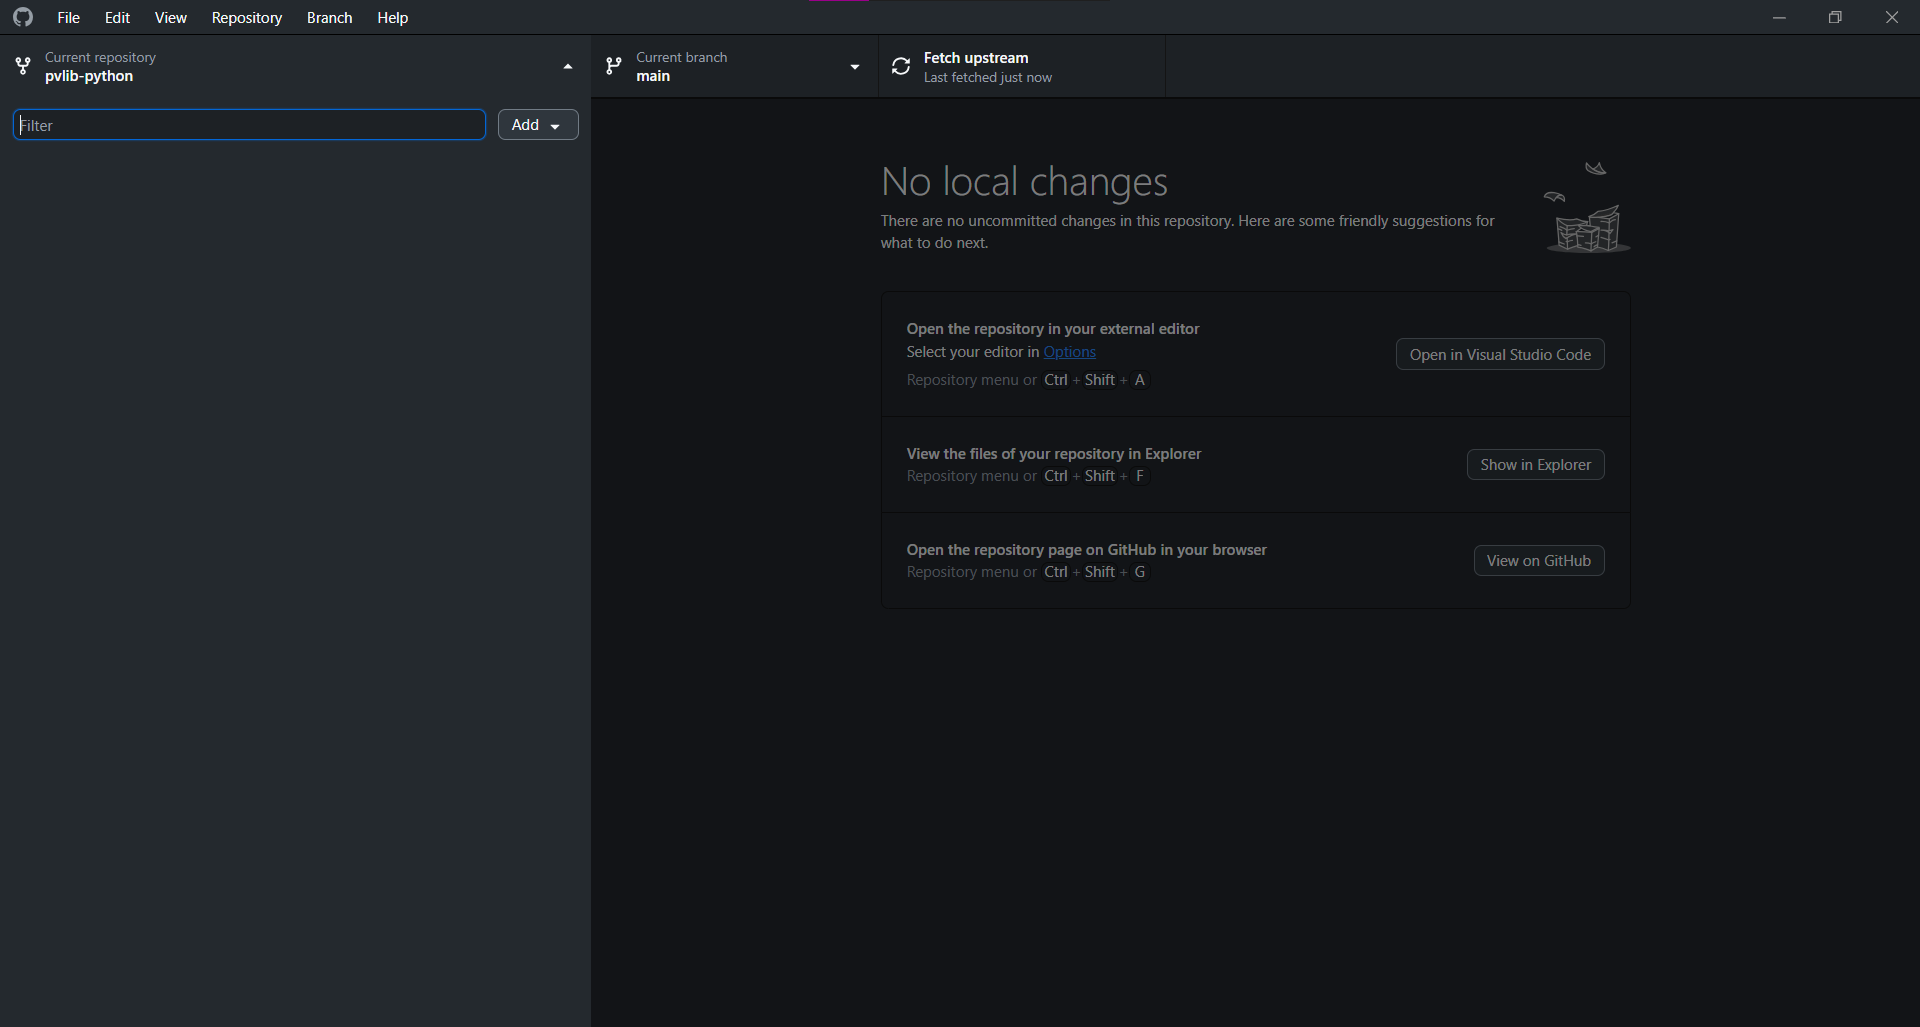
\includegraphics[width=0.6\textwidth]{images/SoA_foss/GH_DKT_0.png}
              \caption{Pantalla principal de GitHub Desktop.}
              \label{fig:GH_principal}
          \end{figure}

    \item A continuación, se crea una \gls{rama} de trabajo específica para los cambios que se vayan a realizar. Se crea pinchando sobre ``Current Branch'' \textrightarrow ``New Branch''.
    \item Ahora se puede abrir la carpeta en la que se ha clonado el repositorio y hacer las ediciones correspondientes.
    \item Una vez hechos los cambios, se añade un mensaje descriptivo de qué se ha cambiado y se pincha en ``Commit to ...''; así los cambios formarán parte de la rama creada. Cada entrada en este historial de cambios se llama \textit{\gls{commit}}.
    \item El botón superior izquierdo indicará ``Push'' cuando hayan cambios en la rama local que no estén publicados en internet. Debe pulsarse.
    \item En este momento se usa la combinación de teclas \texttt{Control+R} para abrir una \textit{\gls{pull request}}. Alternativamente se puede hacer esto mismo desde la web de GitHub.
    \item A partir de aquí se detalla qué se propone y se interacciona con la comunidad de \pvlibpy{} para que revisen la propuesta y decidan si se añaden o no estos cambios.
\end{enumerate}

Otras opciones para contribuir van desde usar \textit{Git} por \gls{línea de comandos}, otros clientes como \textit{SourceTree} o características integradas en los programas de edición de código.

\section{La librería \pvlibpy{}} \label{sct:pvlib}

Antes de proseguir con las contribuciones, es necesario tratar sobre qué es y qué aporta la \gls{librería} \pvlibpy{}.

\pvlibpy{} es una biblioteca de código abierto que proporciona herramientas para la simulación, análisis e investigación de sistemas fotovoltaicos. Se encuentra desarrollada para el lenguaje de programación interpretado \gls{Python} \cite{CS-R9526}, que es ampliamente utilizado en las comunidades científica y de desarrollo de \gls{software} por su gratuidad, sintaxis sencilla, facilidad de desarrollo y diseño orientado a objetos.

Surge como un proyecto independiente a partir de su predecesor escrito en \gls{MATLAB}, \textit{MATLAB\_PV\_LIB}.

La librería \pvlibpy{} aporta una serie de mejoras entre las que destacan la infraestructura de tests, la documentación y otros procedimientos de Integración Continua y Desarrollo Continuo (\textit{CI/CD}) que facilitan el desarrollo. Además, está escrita en un lenguaje de programación libre y gratuito; mientras que \gls{MATLAB} es propietario y de pago. Por el contrario, en \textit{MATLAB\_PV\_LIB} no existen tests, el control de versiones resulta más confuso e inaccesible al estar en un documento de Microsoft Word y, en general, hay falta de mantenimiento\footnote{Véase \url{http://web.archive.org/web/20211207215130/https://pvlib-python.readthedocs.io/en/v0.9.0/comparison_pvlib_matlab.html}.}.

Como todo proyecto de código abierto que se encuentra en constante desarrollo, \pvlibpy{} cuenta con un grupo de desarrolladores y colaboradores que contribuyen a su mantenimiento y mejora continua. Estas personas partícipes del proyecto son mayoritariamente personal dedicado a la ciencia e investigación en diferentes instituciones y universidades públicas, aunque también existe personal de ingeniería e investigación del ámbito privado. El código y la colaboración se realiza a través del repositorio de código abierto en GitHub\footnote{Acceso a través de \url{https://github.com/pvlib/pvlib-python}.}.

El código se encuentra disponible al público bajo la \gls{licencia} \textit{BSD 3-Clause}\footnote{Texto de la licencia disponible en \url{https://opensource.org/license/BSD-3-clause}.}, que permite su uso, modificación, redistribución e integración en otros proyectos siempre que haga la atribución de autoría pertinente y no emplee la imagen de \pvlibpy{} con fines publicitarios o promotores. La librería se distribuye a través del índice de paquetes de Python, PyPI\footnote{Véase \url{https://pypi.org/project/pvlib/}.}, y en el canal de \textit{conda-forge}\footnote{Véase \url{https://anaconda.org/conda-forge/pvlib}.} para la distribución \textit{Conda}, que está orientada a facilitar conjuntos de librerías para ciencia de datos de forma estable y robusta. \textit{Conda} se distribuye en dos \textit{flavours} -sabores o conjuntos de librerías- conocidas como \textit{Anaconda} y \textit{Miniconda}, cada una con sus propias características y ventajas en tiempo de instalación, espacio en disco y paquetes preinstalados.

La \gls{documentación} de la librería\footnote{Accesible en \url{https://pvlib-python.readthedocs.io/en/stable/}} se encuentra disponible en la plataforma\\ \mbox{\textit{ReadTheDocs}}, donde se detallan las funcionalidades, los ejemplos de uso, la estructura del código -la \gls{API}-, las herramientas de desarrollo, las directrices para contribuir al proyecto y la historia de cambios y versiones. La documentación se encuentra disponible exclusivamente en inglés.

\subsection{Objetivos de la librería} \label{ssct:pvlib:objetivos}

Como se ha comentado anteriormente, la \gls{librería} \pvlibpy{} tiene como objetivo principal proporcionar herramientas para la simulación, análisis e investigación de sistemas fotovoltaicos. Para ello, cuenta con una serie de funciones y clases que permiten realizar cálculos de radiación solar, generación de energía, sombreado, eficiencia de módulos y pérdidas de energía, entre otros. Estas herramientas se basan en modelos científicos y algoritmos validados por la comunidad científica y se han implementado en Python para facilitar su uso y extensión. Es importante denotar que los autores pretenden establecer la implementación de la librería como una referencia fiable y certera de los modelos científicos que se emplean en la \gls{simulación} de sistemas fotovoltaicos, poniendo un enfoque especial en la rigurosidad de las publicaciones y de los artículos científicos que se emplean como base.

Enumerando los objetivos de la librería, se pueden destacar los siguientes:

\begin{enumerate}
    \item Proporcionar herramientas para la \gls{simulación} y análisis de sistemas fotovoltaicos.
    \item Implementar modelos científicos y algoritmos validados por la comunidad científica.
    \item Establecer un referente fiable de las implementaciones de las características citadas anteriormente.
    \item Auditar las contribuciones para garantizar la funcionalidad de las aportaciones.
    \item Facilitar la integración con servicios de datos meteorológicos y bases de datos de radiación solar.
    \item Fomentar la colaboración y la contribución de la comunidad científica y de desarrollo de software.
\end{enumerate}

Cabe destacar que también hay fines que la comunidad de \pvlibpy{} excluye como objetivos, es decir, características que no se pretenden implementar o documentar. Entre estos destacan:

\begin{enumerate}
    \item Proporcionar contenido didáctico sobre la energía solar fotovoltaica, más allá del estrictamente necesario para entender y aplicar las utilidades disponibles.
    \item Hacer inferencias, sugerencias o recomendaciones que no estén publicadas formalmente sobre el uso de los modelos implementados.
    \item Facilitar un sistema \textit{ready-to-go} para usuarios finales.
\end{enumerate}

Puede parecer que excluir estos objetivos son limitantes en cuanto a la divulgación y al alcance, pero en realidad se trata de una forma de garantizar la calidad y la fiabilidad de la librería. Así el esfuerzo limitado de los mantenedores y los contribuyentes se centra en la implementación rigurosa de publicaciones de la comunidad científica.

Una nota importante, en especial sobre el último punto, es que la definición de la misma librería es que se trata de una ``caja de herramientas''\footnote{Del inglés, ``toolbox''. \url{https://github.com/pvlib/pvlib-python/blob/99619e8fc5aea5c5dc4dacabb75b617786cc4a1a/README.md?plain=1\#L61}.}, porque es la persona usuaria de la biblioteca es la responsable de generar un flujo de trabajo adecuado para sus fines. Esta nota es en contraposición a las herramientas de simulación y análisis de sistemas fotovoltaicos comerciales, que limitan y simplifican la experiencia del usuario, varias veces dejando de lado la \gls{documentación} y la transparencia de los cálculos\footnote{Como hecho anecdótico, se puede observar alguna crítica sobre esto entre los partícipes del proyecto, por ejemplo en \url{https://github.com/pvlib/pvlib-python/issues/2057\#issuecomment-2197279047}.}.

\subsection{Funcionalidades} \label{ssct:pvlib:funcionalidades}

El proyecto de código abierto \pvlibpy{} cuenta múltiples características que abarcan un amplio rango de temas relacionados con la producción de energía solar fotovoltaica. Al momento de la redacción de este documento, la versión de la librería es la 0.11.0, publicada el 21 de junio de 2024. A continuación, se detallan algunas de las funcionalidades más destacadas:

\begin{itemize}
    \item Cálculo de la posición del sol: para determinar la posición del sol en el cielo en función de la localización y la hora del día, en el \gls{submódulo} \texttt{pvlib.solarposition}.
    \item Cálculo de valores estándares de la radiación solar: la librería proporciona herramientas para calcular la \gls{radiación solar} en una superficie plana y horizontal en función de la localización, la posición del sol y parámetros atmosféricos. Véase \texttt{pvlib.solarposition} y \texttt{pvlib.clearsky}.
    \item Procedimientos de descomposición, \gls{transposición} y \gls{transposición inversa} de la radiación solar: se emplean para, a partir de la irradiance solar en una superficie plana y horizontal, obtener la incidente en un colector plano orientado arbitrariamente. Y una vez obtenidas las componentes \gls{directa}, \gls{difusa} y de \gls{albedo} de esta irradiancia, aplicar correcciones convenientes para obtener la radiación efectiva colectada en la superficie. También se puede realizar el proceso inverso, de las componentes en el plano inclinado a la radiación en una superficie plana y horizontal. Estas utilidades se encuentran en el submódulo \texttt{pvlib.irradiance}.
    \item Obtención de parámetros atmosféricos como la columna o masa de aire, un número que representa cuánta atmósfera hay, relativa a la columna completamente vertical (\texttt{AM=1}), en el submódulo \texttt{pvlib.atmosphere}.
    \item Valores de \gls{albedo} predefinidos, bien de materiales sólidos o de superficies naturales de agua, en \texttt{pvlib.albedo}.
    \item Corrección de la radiación incidente en función del ángulo de incidencia (\gls{IAM}): debido a la reflexión que sufre la luz solar al incidir en una superficie de forma oblicua. Las utilidades se encuentran en el submódulo \texttt{pvlib.iam}.
    \item Producción fotovoltaica: mediante puntos característicos como el de máxima potencia (\textit{MPP}) o calculando curvas I-V completas. Se emplean modelos de eficiencia de módulos y pérdidas de energía para estimar la producción de energía en un sistema fotovoltaico, mediante el modelo de un único \gls{diodo}. Se encuentra en el submódulo \texttt{pvlib.singlediode}.
    \item Cálculo de sombreado: métodos analíticos para calcular la fracción sombreada de hileras de filas. Véase el submódulo \texttt{pvlib.shading}.
    \item Cálculo de ángulos de seguimiento: para seguidores de uno y dos ejes, que permitan colectar la máxima radiación solar \gls{directa}, que normalmente se corresponderá con la máxima producción de energía. Véase el submódulo \texttt{pvlib.tracking}.
    \item Cálculo de temperatura de los módulos: normalmente empíricos, facilitan estimar la producción de energía ya que, habitualmente, la eficiencia de las células es bastante susceptible a la temperatura. Estas utilidades se encuentran en \texttt{pvlib.temperature}.
    \item Estimación de ganancias o pérdidas por efectos del espectro solar: pues en función de la composición del espectro solar incidente en los módulos, la eficiencia de los mismos puede variar. En \texttt{pvlib.spectrum}.
    \item Modelado de eficiencia de inversores: para estimar la eficiencia de los \gls{inversores} DC-AC en función de la potencia de entrada y sus demás características. En \texttt{pvlib.inverter}.
    \item Modelado de pérdidas en transformadores: para estimar las pérdidas en los \gls{transformadores} de conexión a red. En \texttt{pvlib.transformer}.
    \item Modelado de pérdidas en cables: para estimar las pérdidas resistivas en los cables. En \texttt{pvlib.pvsystem}.
    \item Integración de APIs externas para la obtención de datos meteorológicos relacionados con la fotovoltaica, en \texttt{pvlib.iotools}.
    \item Abstracciones de los componentes que conforman una instalación fotovoltaica, mediante las clases \texttt{Location}, \texttt{Array}, \texttt{PVSystem} y la clase que agrupa el flujo computacional \texttt{Modelchain}, en los submódulos \texttt{pvlib.location}, \texttt{pvlib.pvsystem} y \texttt{pvlib.modelchain}.
    \item Cálculos adicionales para sistemas con \gls{módulos bifaciales}, que son aquellos \gls{colectores} planos que permiten la captación de radiación solar por ambas caras del módulo. En \texttt{pvlib.bifacial}.

\end{itemize}

\subsection{Repositorio del proyecto} \label{ssct:pvlib:repositorio}

Como se ha mencionado anteriormente, el código de la librería \pvlibpy{} se encuentra alojado en un \gls{repositorio} de código abierto. Un repositorio es una carpeta que contiene una series de archivos, de los cuales los más importantes se gestionan mediante un sistema de control de versiones (\gls{VCS}). Este sistema permite llevar un registro de los cambios realizados en los archivos, así como la posibilidad de volver a versiones anteriores en caso de que se produzca un error o un fallo en el código. El uso de esta herramienta es indispensable en proyectos de software, ya que facilita la colaboración entre los desarrolladores y la gestión de las versiones del código.

En el caso de \pvlibpy{}, el repositorio se encuentra alojado en la plataforma GitHub, que es una de las más populares para el alojamiento de proyectos de código abierto.

El repositorio cuenta con múltiples archivos y sub-carpetas que configuran el proyecto. Algunos de los más destacables son:

\begin{itemize}
    \item \texttt{README.md}: es el primer archivo en verse en la plataforma online y contiene la descripción del proyecto, su propósito y cómo instalarlo, entre otros.
    \item \texttt{LICENSE}: es el archivo que contiene la \gls{licencia} del proyecto, en este caso la licencia \textit{BSD 3-Clause}.
    \item \texttt{pyproject.toml}, \texttt{setup.cfg}, \texttt{setup.py}, \texttt{MANIFEST.in}: son los archivos que definen la configuración del proyecto, como el nombre, la versión, la descripción, las dependencias, los archivos que componen una distribución precompilada o de código fuente, etc. que las personas usuarias verán en la plataformas de distribución de paquetes.
    \item \texttt{docs/}: es la carpeta que contiene archivos de configuración y explicativos que permiten generar la documentación del proyecto. No obstante, el código que se expone públicamente se documenta automáticamente a partir de unos comentarios en el código.
    \item \texttt{pvlib/}: es la carpeta que contiene el código fuente de la librería, organizado en sub-carpetas y archivos según su funcionalidad. Los tests unitarios y de integración se encuentran en esta carpeta.
    \item \texttt{AUTHORS.md}, \texttt{CODE\_OF\_CONDUCT.md}, \texttt{codecov.yml}, \texttt{readthedocs.yml}, \texttt{paper/}, \texttt{ci/}, \texttt{benchmarks/} y \texttt{.github/}: son archivos y carpetas que contienen información adicional sobre el proyecto y la configuración de todos los flujos de integración continua: destacan los tests, los benchmarks y la documentación.

\end{itemize}

\subsection{Frameworks de desarrollo del proyecto} \label{sct:pvlib:dev}

Como tal, el desarrollo del proyecto requiere el conocimiento de algunas herramientas que permiten la colaboración con el repositorio principal y cumplir con las directrices para contribuir al proyecto. Estas se suelen denominar \textit{frameworks} de desarrollo, literalmente marcos de trabajo, que normalizan la forma de desarrollar y colaborar en el proyecto.

La elección de las herramientas empleadas corresponde a una preferencia en cuanto a uso y extensión en el desarrollo software, pero pueden variar en el futuro, como ya lo ha hecho en el pasado.

En el lado de las utilidades esenciales, se encuentran:

\begin{itemize}
    \item \textit{Git}: como sistema de control de versiones (\gls{VCS}) que se emplea para gestionar los cambios en el código.
    \item \textit{GitHub}: es la plataforma de alojamiento de proyectos de código abierto que se emplea para colaborar en el desarrollo del proyecto. Permite crear \textit{issues} o discusiones para reportar errores o sugerir mejoras; y proponer cambios y revisarlos públicamente en \textit{pull requests}. Además proporciona máquinas virtuales para ejecutar los procedimientos de integración y desarrollo continuos.
    \item \textit{ReadTheDocs} junto con \textit{sphinx}: es la plataforma que se emplea para ejecutar \textit{sphinx}, el entorno de trabajo que produce la documentación en formato \gls{HTML}, y alojar el producto. La documentación se escribe en formato \textit{\gls{reStructuredText}} y se genera automáticamente a partir de los comentarios en el código, \gls{scripts} con los ejemplos y archivos fuente con el cuerpo más general.
    \item \textit{pytest}: es la librería de \gls{Python} que se emplea para escribir y ejecutar tests unitarios y de integración en el código. Facilita la creación de \textit{\gls{mocks}} u observadores del estado de partes del mismo proyecto, la reutilización de datos de tests, la ejecución opcional de los tests en función de las dependencias disponibles y visualizar los resultados en un informe. Posiblemente la mejor característica es poder ejecutar los tests uno a uno, por grupo o todos a la vez.
    \item \textit{Codecov}: es la plataforma que se emplea para medir la cobertura de los tests en el código. Permite visualizar la cobertura de los tests en un informe y comprobar si se están realizando pruebas suficientes en el código.
    \item \textit{flake8}: es una utilidad que detecta errores de estilo en el código, como la longitud de las líneas, la \gls{indentación}, la presencia de espacios en blanco, entre otros. Facilita la escritura de código limpio y legible, por ende, mantenible.
          Además, facilita la detección de errores estáticos en el código; esto es, condicionales que nunca se cumplen, variables que no se usan, importación innecesaria de módulos, identificadores duplicadas o que no siguen la convención de nombres, entre otros.

\end{itemize}

\section{Entorno de desarrollo y herramientas utilizadas} \label{sct:desarrollo:entorno}

Para el desarrollo de este trabajo se emplea el siguiente \gls{software} para el desarrollo del proyecto consistentemente a lo largo de toda su ejecución:

\begin{itemize}
    \item \textit{Visual Studio Code}: es el editor de código que se emplea para escribir y editar el código fuente del proyecto. Es un editor de código semi-abierto, ligero y rápido que cuenta con una amplia gama de extensiones para facilitar el desarrollo de software. Es una alternativa multipropósito a otros editores de código como \textit{PyCharm} o \textit{Spyder} en el caso de \gls{Python}. Es multipropósito en cuanto admite el desarrollo de muchísimos lenguajes de programación y sintaxis de ficheros ampliamente utilizados en el desarrollo software.

          A continuación se muestra una captura de pantalla de \textit{Visual Studio Code} con algunos ficheros usados en la implementación de la propuesta \href{https://github.com/pvlib/pvlib-python/pull/2070}{\#2070}:

          \begin{figure}[H]
              \centering
              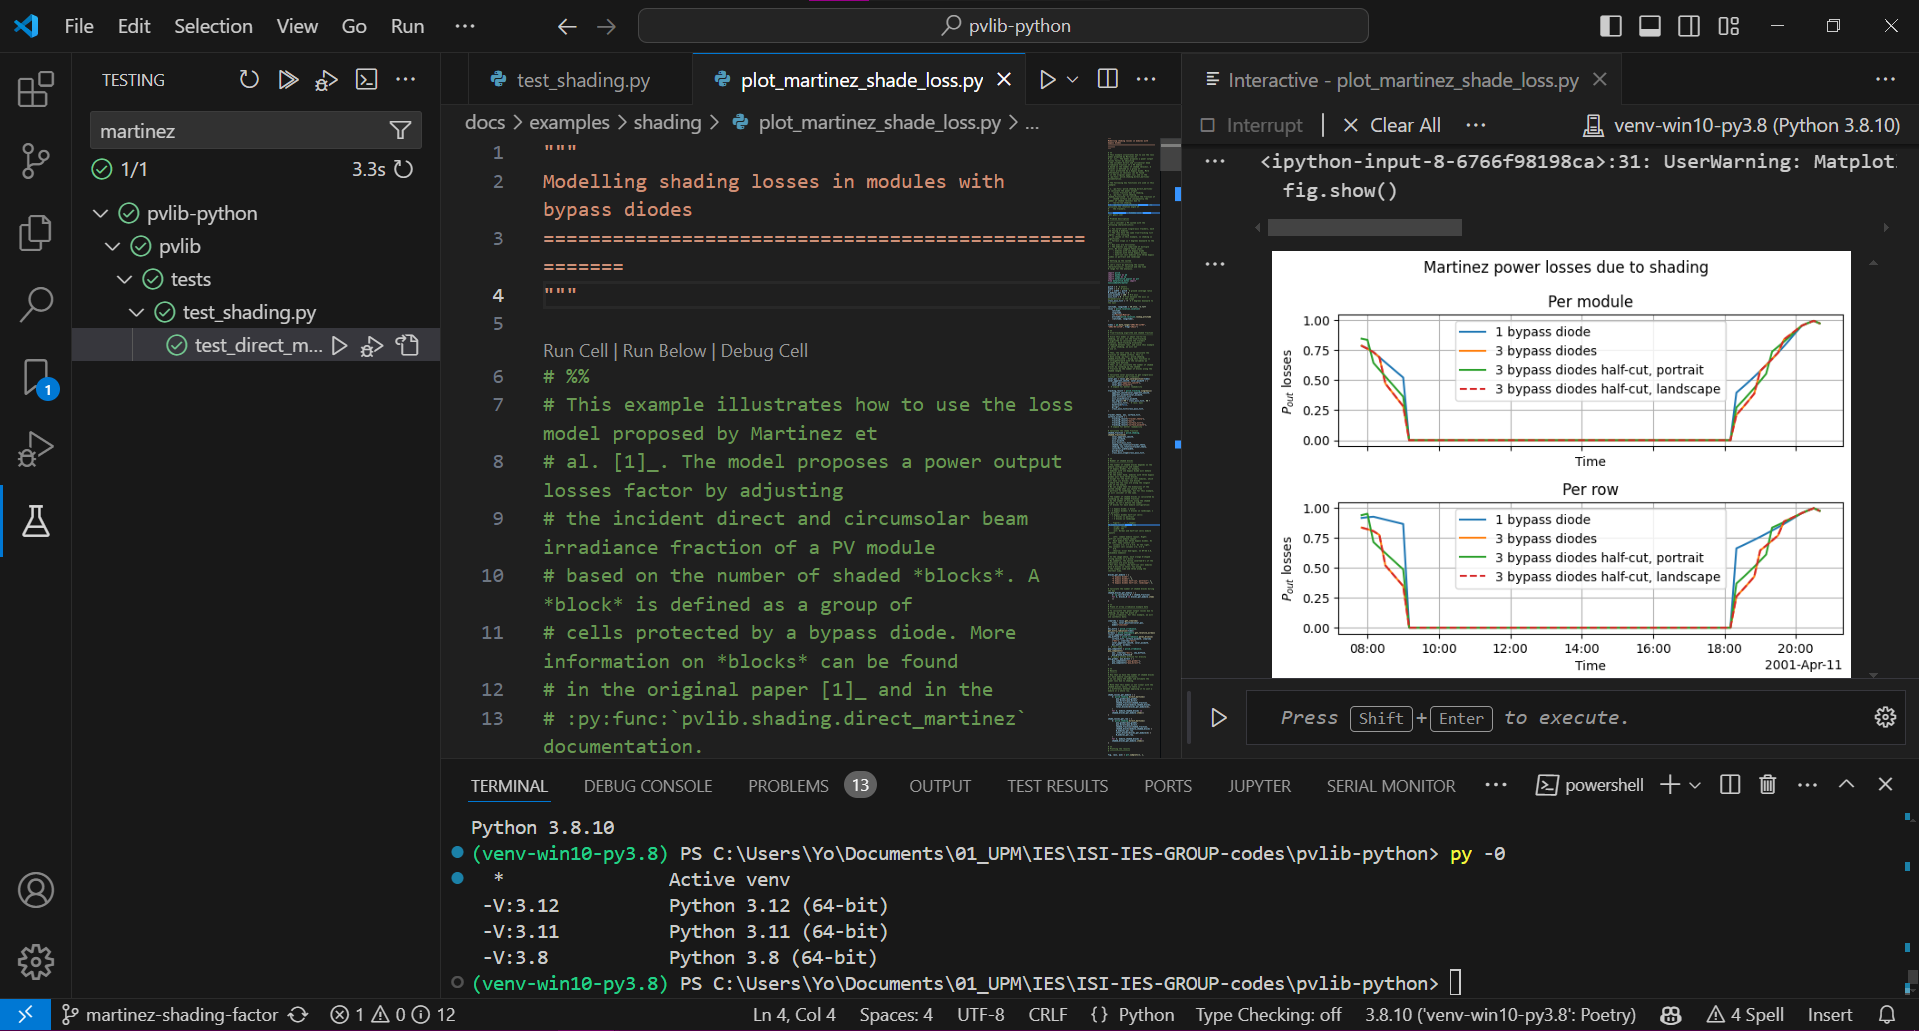
\includegraphics[width=0.9\textwidth]{./images/SoA_foss/VSCode.png}
              \caption{Captura de pantalla de \textit{Visual Studio Code} con algunos ficheros usados en \ref{sct:desarrollo:contribuciones_cientificas:perdidas_sombreado}.}
              \label{fig:vscode}
          \end{figure}

          Es importante denotar que la inmensa utilidad que proporciona \textit{VSCode} es gracias a las extensiones creadas por la comunidad de desarrolladores, que permiten desde la edición de archivos de texto plano hasta la depuración del código, pasando por la integración con servicios de control de versiones y la ejecución de tests desde la interfaz.

          A continuación se detallan extensiones que se emplean en el desarrollo del proyecto:

          \begin{itemize}

              \item \textit{Python}: es la extensión que se emplea para el desarrollo de código en Python. Proporciona funcionalidades como el autocompletado de código, la visualización de la documentación de las funciones, la ejecución de scripts y la depuración de código.
              \item \textit{Ruff}: permite formatear el código según las directrices de estilo de \textit{flake8}, la utilidad que da estilo uniforme al código de Python. Se recuerda que establece limitaciones en cuanto a la longitud de las líneas y a la forma de escribir todo el código.
              \item \textit{GitHub Copilot}: un asistente de generación de código en línea integrado en el editor, que se emplea para sugerir fragmentos de código y documentación en función del contexto. Agiliza el desarrollo.
              \item \textit{Code Spell Checker}: es un corrector ortográfico que se emplea para detectar errores de ortografía en el código y en la documentación.
              \item \textit{Jupyter Notebooks}: es la extensión que se emplea para editar y ejecutar \textit{notebooks} de Jupyter en el editor, un formato que permite visualizar las variables del contexto y facilita el \gls{debugging} interactivo. Los ejemplos de \pvlibpy{} se realizan con un formato similar a las celdas de texto o código de una \textit{notebook}.
              \item Resaltado de sintaxis de varios formatos de archivos, como \textit{\gls{reStructuredText}}, \textit{Markdown}, \textit{YAML} y \textit{TOML}: para facilitar la edición de la documentación y los archivos de configuración.

          \end{itemize}

    \item \textit{GitHub Desktop}: es la \gls{interfaz gráfica} que se emplea para colaborar en el desarrollo del proyecto. Permite visualizar los cambios, crear \textit{ramas}, hacer \textit{commits}, \textit{pull requests} y \textit{\gls{merges}}, entre otros. En resumen, administra nuestra copia del repositorio para que los desarrolladores del proyecto puedan revisar y aceptar las propuestas.
    \item \textit{pip} y \textit{venv}: como gestor de paquetes y entornos aislados de desarrollo de Python nativos. Se emplean para instalar las dependencias del proyecto y usar entornos con las versiones específicas requeridas aislado del resto del sistema.

\end{itemize}

De forma discreta, se ha hecho uso de otras herramientas como:

\begin{itemize}
    \item \textit{Git}: para \gls{clonar} las ramas con los cambios planteados en este TFG y ejecutar partes de la integración continua, normalmente la documentación, en las máquinas virtuales de linux provistas por la UPM\footnote{Accesible a través de \url{https://escritorio.upm.es/}.}.
    \item \textit{Miniconda}: una distribución de Python que se emplea para instalar y gestionar las dependencias del proyecto. Facilita la creación de entornos virtuales y la instalación de paquetes de Python. Se utilizó para diagnosticar un error de precisión por la compilación de algunas librerías y que hacía fallar un test.
    \item \textit{LibreOffice Calc}: para generar datos de prueba y comprobar las implementaciones de las ecuaciones de los modelos.
\end{itemize}

El desarrollo de la librería se ha hecho habitualmente en un portátil con Windows 10 así que se ha aprovechado a usar el subsistema de Windows para Linux (\textit{WSL}) para ejecutar tests y construir la documentación en un entorno similar al de integración continua ocasionalmente. No obstante, por los recursos limitados que ofrece un portátil, y por desear cambiar de ramas mientras los procedimientos de integración continua se efectúan, se ha hecho uso de las máquinas virtuales de la UPM para construir la documentación y analizar algún test.

\section{La documentación}

En esta sección se pondrá en valor lo que realmente es lo más importante de un proyecto de programación, en especial de código abierto: la \gls{documentación}. Es más, se puede argumentar que el valor de todas las aportaciones es documentar lo más rigurosamente posible los modelos y métodos que se implementan, tanto para facilitar su correcto uso como para divulgar su existencia y problemática que resuelven.

Que una buena documentación respalde un proyecto de código abierto es crítica para el éxito del mismo \cite{Imani_Radmanesh_Ahmed_Moshirpour_2024}. Es la carta de presentación a público interesado, y es la guía de uso para las personas usuarias. El caso inverso es una documentación pobre, que puede llevar a la confusión y a la desconfianza en la calidad del software.

Como se comentaba anteriormente, la documentación de la librería \pvlibpy{} se encuentra alojada en la plataforma \textit{ReadTheDocs}, que expone los archivos HTML para que las personas usuarias puedan consultarla en línea. La documentación se genera automáticamente a partir de los comentarios escritos en el código fuente, que se escriben en formato \textit{\gls{reStructuredText}} y se construye con el \gls{framework} \textit{sphinx}.

Existen archivos específicos para indicar qué funciones o métodos son públicos, hacer páginas de inicio, de referencia, de ejemplos, de instalación, de contribución, etc. Además, se pueden incluir imágenes, tablas, gráficos, enlaces, referencias, entre otros elementos que facilitan la comprensión de los conceptos.

\textit{Sphinx} emplea el estilo de documentación de \textit{pydata-sphinx-theme}, que organiza las secciones de la documentación y da un estilo homogéneo a la web. Además, para la creación de los ejemplos se emplea la extensión \textit{sphinx-gallery}, que ejecuta unos scripts de Python por secciones similares a una \textit{notebook} de Jupyter y captura la salida de texto \gls{estándar} y los gráficos para mostrarlos en la documentación.

La \textit{\gls{docstring}} de cada \gls{función}, que es el comentario que se escribe en la primera línea de la definición de la función y se emplea para autogenerar la documentación, utiliza el estilo de \textit{numpydoc}. Este estilo permite incluir información sobre los parámetros de entrada, los \gls{valores de retorno}, las excepciones que se pueden lanzar, entre otros. Además, se pueden incluir ejemplos de uso de la función e informar avisos de precaución sobre aspectos más específicos.

A continuación se muestra como ejemplo una función mínima con su plantilla de documentación y de código de una función escrita con este fin:

\begin{lstlisting}[language=Python, caption={Ejemplo de documentación de una función en \pvlibpy{}.}, label={lst:doc_function_example}]
def example_model(param1, param2):
    """
    Brief model description.

    Long model description, also found at [1]_.

    .. versionadded:: 0.1.0

    .. warning::
       This docstring is an example.

    Parameters
    ----------
    param1 : numeric
      Description of the parameter.
    param2 : numeric
      Description of the parameter.

    Returns
    -------
    float
        Return type of the function.

    Notes
    -----
    Additional notes about the function, detailed explanations if needed. Even an equation:

    .. math::

       f(x, y) = x + y

    Examples
    --------
    >>> example_model(1, 5)
    6.0

    References
    ----------
    .. [1] Author, A. (2024). Title of the paper. Journal, 1(1), 1-10. :doi:`10.0001/populate`
    """
    return float(param1 + param2)
\end{lstlisting}

Esta \gls{función}, una vez listada en el archivo correspondiente del índice que nos interese -aquí usamos el \gls{submódulo} \texttt{pvlib.solarposition} como ejemplo-, creará una página como la que se muestra en la figura \ref{fig:doc_function_example}:

\begin{figure}[H]
    \centering
    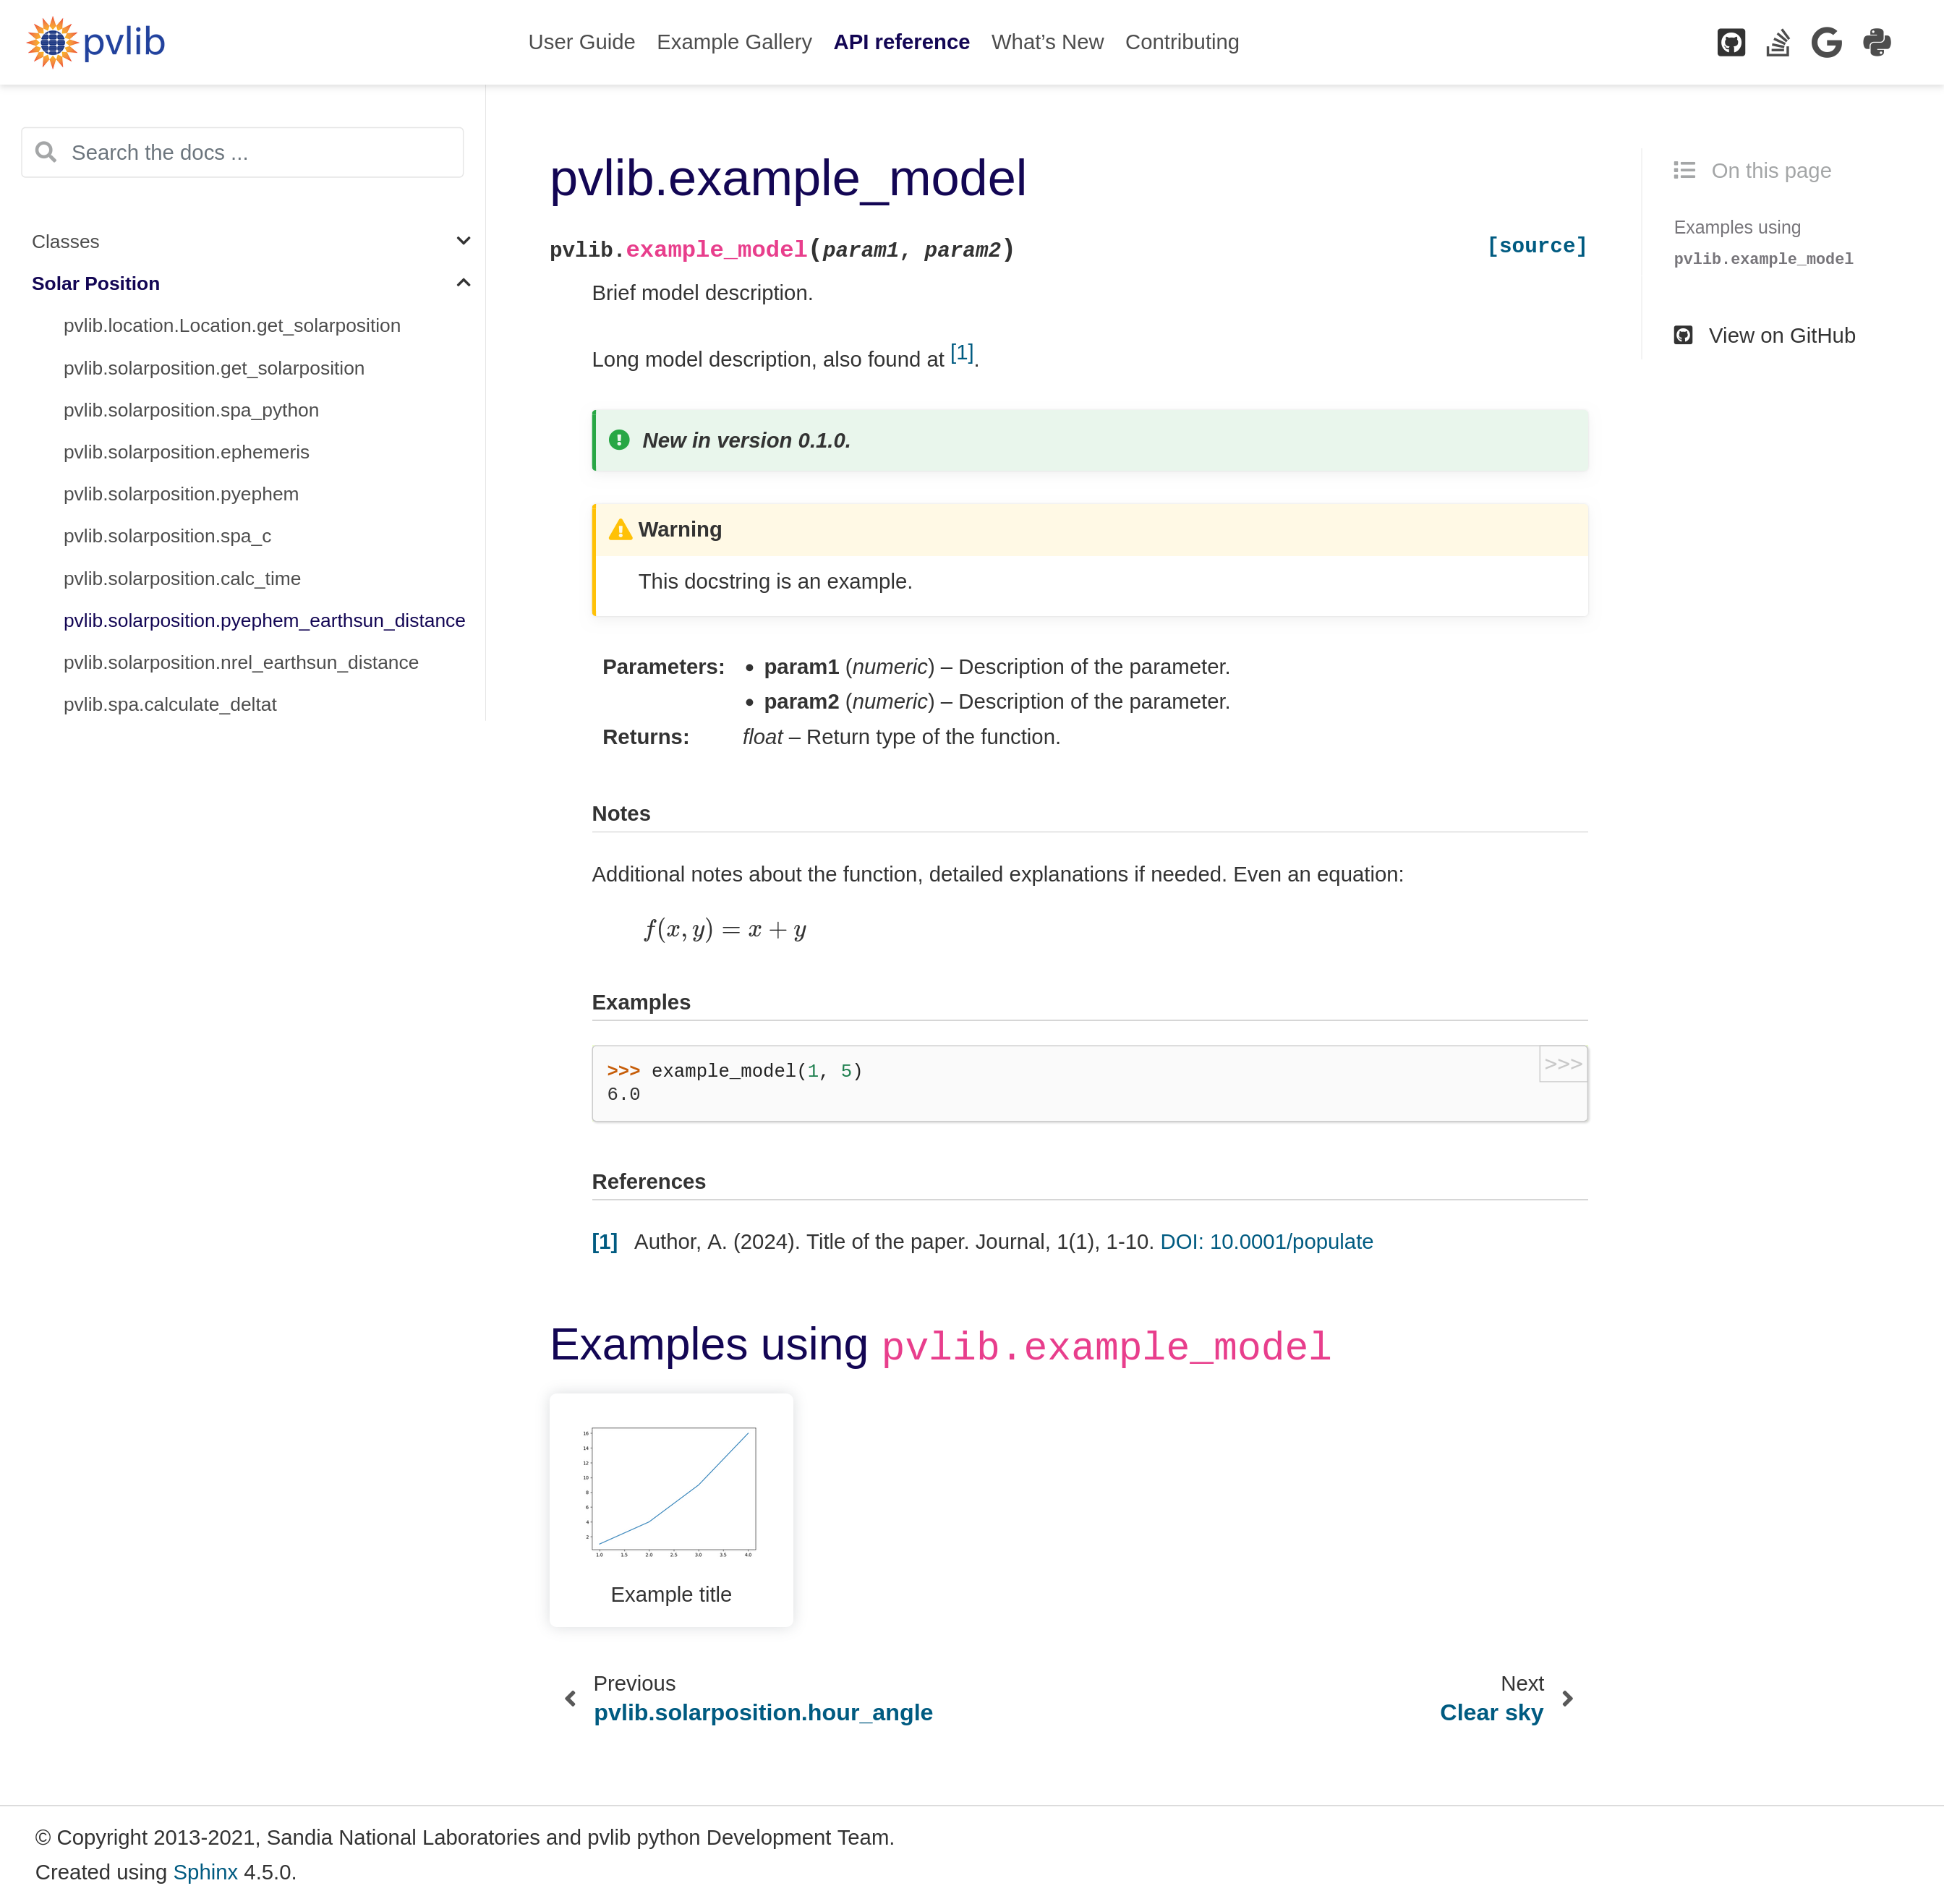
\includegraphics[width=0.8\textwidth]{./images/how_to_document/function_stretch.png}
    \caption{Un ejemplo de renderizado de la documentación de una función en \pvlibpy{}.}
    \label{fig:doc_function_example}
\end{figure}

Por otro lado, la siguiente estructura pertenece a la redacción de un ejemplo en la documentación. Se emplea para mostrar cómo se usa una \gls{función} dentro de un contexto más elaborado en cuanto a variables de entrada y salida. Puede incluir todas las características de la documentación de una función:

\begin{lstlisting}[language=Python, caption={Plantilla para elaborar un ejemplo en \pvlibpy{}.}, label={lst:how_to_document_example}]
"""
Example title
=============

Brief model description (shown in preview card).
"""

# %%
# Text paragraph, in reStructuredText format. Can use sections, subsections, etc., and math as in LaTeX.
# More text.

# This is a comment (there is a newline above)
import matplotlib.pyplot as plt
from pvlib import example_model
print("Hello, world!")
plt.plot([1, 2, 3, 4], [1, 4, 9, 16])
plt.show()

# %%
# Return to paragraph text.

sum_val = example_model(1, 5)
print(f"Sum of 1 and 5 is {sum_val}.")
\end{lstlisting}

El texto anterior constituye un archivo que, ubicado en la carpeta correcta (aquí el archivo es \texttt{docs/examples/solar-position/example\_example.py}), hará que se cree automáticamente una página como la que se muestra en la Figura \ref{fig:doc_use_example}.

\begin{figure}[H]
    \centering
    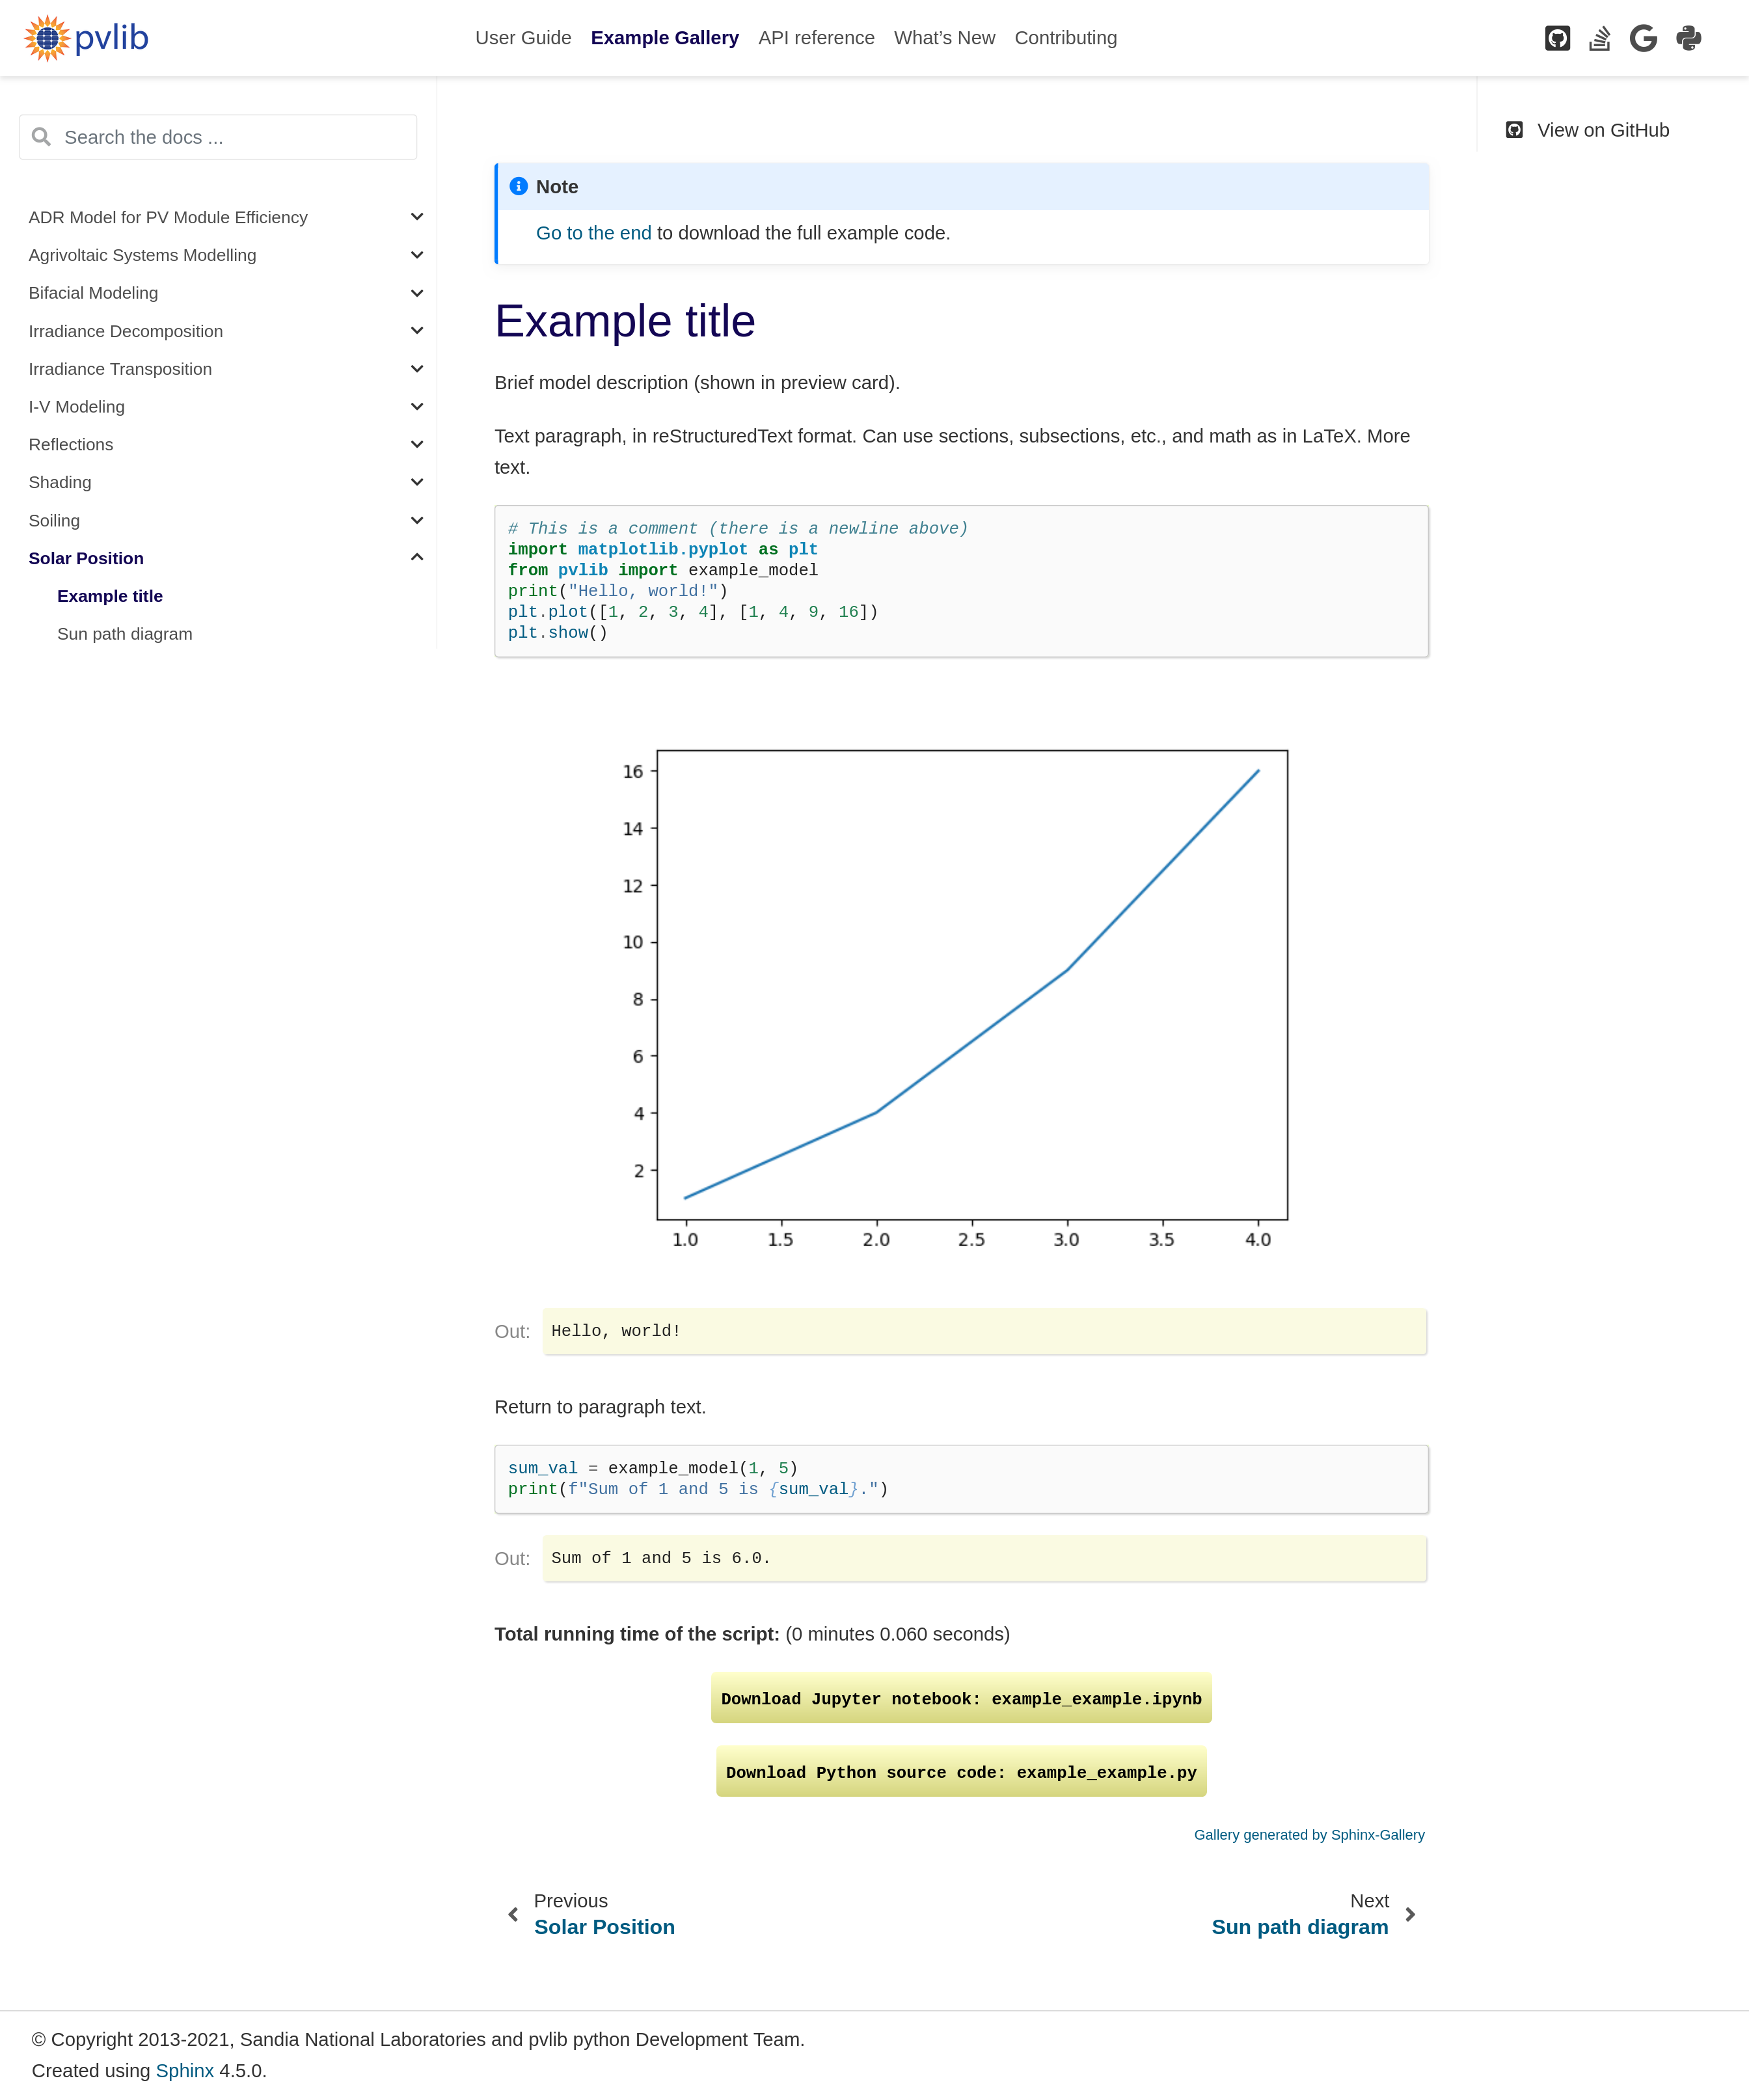
\includegraphics[width=0.9\textwidth]{./images/how_to_document/example_stretch.png}
    \caption{Un ejemplo de uso en la documentación de \pvlibpy{}.}
    \label{fig:doc_use_example}
\end{figure}

Por último queda construir la documentación. A continuación se muestran los comandos que deben ejecutarse para este fin:

\begin{itemize}
    \item En un sistema basado en \textit{Linux} o \textit{WSL}.
    \item Clonando el repositorio original de la librería con \textit{Git}.
    \item Empleando las mismas versiones que a día de la redacción de este documento se emplea en la integración continua (\textit{pvlib-python=0.11.0}) - en especial hay que hacer la instalación de Python3.8.
    \item Con el entorno aislado de desarrollo (\textit{venv}) activado.
    \item Y realizando una instalación local mediante \textit{pip}.
\end{itemize}

\begin{lstlisting}[language=bash, caption={Comandos para construir la documentación de \pvlibpy{}.}, label={lst:doc_build}]
# instalar Python 3.8 desde el repositorio de deadsnakes,
# en las librerias por defecto de Ubuntu no se encuentra disponible por antiguedad
sudo add-apt-repository ppa:deadsnakes/ppa -y
sudo apt-get update
sudo apt-get install python3.8 python3.8-venv -y

# clonar el repositorio de pvlib-python
git clone https://github.com/pvlib/pvlib-python
cd pvlib-python

# crear el entorno virtual, instalar pvlib y las dependencias de la documentacion
python3.8 -m venv .venv
source .venv/bin/activate
python3.8 -m pip install .[doc]

# construir la documentacion
cd docs/sphinx
make html

# abrir la documentacion en el navegador
xdg-open build/html/index.html
\end{lstlisting}

Este conjunto de comandos ha sido ampliamente utilizado para la construcción de la documentación en entornos remotos y así aligerar la utilización de recursos en el portátil personal.

\section{Tests y estrategias de comprobación}

La existencia de tests en un proyecto que se somete a ciclos de continuado desarrollo son esenciales para garantizar el buen funcionamiento ante nuevas versiones de las dependencias y de Python, así como para identificar errores al realizar nuevas implementaciones.

Existen múltiples formas de hacer tests: en especial los unitarios y los de integración son los que se encuentran en proyectos que aglutinan herramientas y procedimientos como en el caso de \pvlibpy{}:

\begin{itemize}
    \item \textit{Tests unitarios}: comprueban que cada \gls{función} o método logra realizar su tarea correctamente. Son los que se aplican a funciones que funcionan por cuenta ajena siempre, y verifican que numéricamente se obtienen resultados adecuados y se lanzan excepciones ante eventos irrealizables.
    \item \textit{Tests de integración}: se utilizan en el flujo de trabajo orientado a objetos que plantea la librería y comprueban que se distribuyen los datos a otras funciones adecuadamente, sin importar tanto el resultado numérico. En este caso, se suelen usar otros objetos que simulan el comportamiento de los objetos reales o vigilan el estado de los mismos.
\end{itemize}

En el caso de \pvlibpy{}, los tests se encuentran en la carpeta \texttt{pvlib/tests/} y se organizan en ficheros y otras carpetas en función de los archivos a los que pertenezcan las funcionalidades a comprobar. Se emplea la librería \textit{pytest} como herramienta de trabajo, que facilita la escritura de tests y permite ejecutarlos individualmente.

Es recomendable aplicar una \gls{estrategia de comprobación} adecuada a cada nueva funcionalidad en desarrollo. Por estrategia de comprobación se indica la forma de abordar qué valores numéricos o eventos deben ocurrir en la ejecución de una \gls{función} bajo test. A veces, será recomendable contar con resultados numéricos obtenidos previamente mediante \gls{hojas de cálculo} u otras implementaciones existentes y disponibles públicamente. En otras ocasiones, se deberá comprobar la ejecución de la función en el contexto de ejecución.

Para el desarrollo de este trabajo, que abarca varios tipos de contribuciones, se ha optado por una estrategia particular a cada propuesta. Normalmente, si la situación lo permite, se ha optado por la comprobación a partir de hojas de cálculo, en alguna ocasión acompañado por la comparación con implementaciones en la misma u otras librerías. Las situaciones que no permiten abordar los tests con esta clase de comprobación se debe a que son problemas que se resuelven de forma más sencilla.
